\chapter{Processi di sviluppo}
\label{chap:processi}
\section{Prospettive sul Processo}
Ogni processo di sviluppo può essere definito attraverso quattro prospettive differenti:
\subsection{Activity perspective}
\textbf{Domanda:} cosa deve essere fatto? \\
La \textbf{Activity Perspective} definisce le attività elementari che vanno a definire il processo. Ogni attività è definita in termini di input, output, condizioni di avvio e condizioni di completamento.
\subsection{Workflow perspective}
\textbf{Domanda:} in che ordine devono essere svolte le attività? \\
La \textbf{Workflow perspective} definisce la sequenza logica e temporale in cui vengono svolte le attività e le possibili alternative.
\subsection{Data-flow perspective}
\textbf{Domanda:} che {artefatto} produce ogni attività? \\
La \textbf{Data-flow perspective} (o \textbf{Artifact perspective}) definisce la sequenza di artefatti che vengono prodotti dal processo.
\subsection{Role-action perspective}
\textbf{Domanda:} chi fa cosa? \\
La \textbf{Role-Action perspective} individua team o persone incaricate di una determinata mansione.
\section{Modelli di processo}
I \textbf{modelli di processo} sono rappresentazioni schematiche o documentate dei flussi di lavoro necessari allo sviluppo di un sistema. Sono da immaginarsi come un'astrazione dei processi. 
\subsection{Modello a cascata}
Il \textbf{modello a cascata} (o \textbf{waterfall}) è un modello di processo sequenziale e lineare, in cui ogni fase del processo deve essere terminata prma di passare alla successiva, senza possibilità di tornare indietro. Il suo nome deriva dal caratteristico \hyperref[appendix:gantt]{Diagramma di Gantt}.
\begin{figure}[h]
    \centering
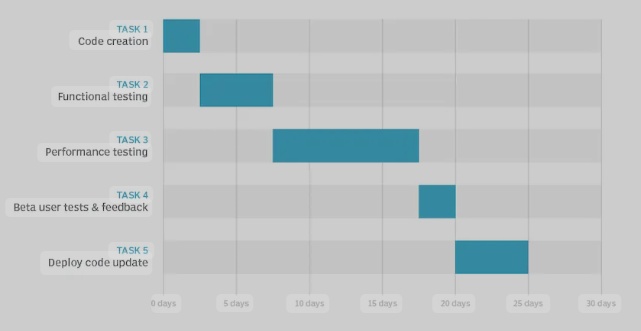
\includegraphics[width=0.75\linewidth]{IDSTEORIA//Immagini/ProcessoUnificato/GanttWaterfall.png}
    \caption{Esempio di diagramma di Gantt in un processo waterfall}
    \label{fig:ganttwaterfall}
\end{figure}
\paragraph{Vantaggi} Struttura semplice e di facile gestione, chiarezza nella documentazione e nelle fasi, adatto a progetti con requisiti ben definiti e stabili.
\paragraph{Svantaggi} Poco flessibile ai cambiamenti, feedback degli stakeholder quasi totalmente ignorato, non adatto a progetti complessi o inesplorati.
\subsection{Modello evolutivo}
Il \textbf{modello evolutivo} è un modello di sviluppo in cui il prodotto viene costruito e migliorato progressivamente, seguendo il feedback degli utenti coinvolti. Si procede per versioni (\textbf{prototipi}) gradualmente sempre più completi. E' anche possibile realizzare prototipi col presupposto di cestinarli (\textbf{Throwaway prototyping}).
\paragraph{Vantaggi} Alta flessibilità, feedback costanti, rischio di fallimento ridotto.
\paragraph{Svantaggi} Possibile progettazione incompleta, difficile fare stima di costi e tempistiche.
\subsection{Modelli Model-Driven}
I \textbf{modelli model-drive} si basano sull'idea di sviluppare software partendo da modelli astratti, che poi vengono trasformati automaticamente o semi-automaticamente in codice eseguibile. 
\paragraph{Vantaggi} Scrittura del codice ridotta, riusco, coerenza e documentazione automatica favorite, manutenibilità più facile.
\paragraph{Svantaggi} Richieste strumenti e competenze specifiche, complessità iniziale, tool non sempre perfetti. 
\subsection{Modelli iterativi}
\label{process-model:iterativi}
I \textbf{modelli iterativi} si pongono a metà tra i modelli a cascata e i modelli evolutivi. Prevedono lo sviluppo attraverso ripetizioni cicliche di mini-waterfall (dette \textbf{iterazioni}). In ogni iterazione si affrontano tutte le fasi del ciclo di vita, ma su un sottoinsieme limitato di requisiti. Alla fine di ogni iterazione il processo viene posto sotto valutazione degli {stakeholder} \\
\paragraph{Vantaggi} Miglioramento continuo, facilità di correzione di errori, adattabilità ai cambiamenti nei requsiti.
\paragraph{Svantaggi} Richiede maggior coinvolgimento del cliente, potenziale aumento dei costi. 
\paragraph{Baseline}
\label{concept:baseline}
Alla fine di ogni iterazione si genera un'insieme di {artefatti} rivisti e approvati chiamati \textbf{baseline}.
\paragraph{Rilascio incrementale}
\label{concept:rilascio-incrementale}
La differenza tra la {baseline} dell'iterazione $n$ e quella dell'iterazione $n-1$ viene chiamata \textbf{incremento}. Ad ogni incremento c'è un rilascio, interno od esterno, che permette di ottenere immediatamente il feedback da parte degli attori coinvolti ed adattare le future iterazioni di conseguenza. Questo processo prende il nome di \textbf{rilascio incrementale}.
\paragraph{Sviluppo a spirale}
\label{concept:sviluppo-spirale}
In ogni iterazione vengono affrontati nuovi requisiti, si affinano le soluzioni e si riduce progressivamente l'incertezza, cercando di mitigare i rischi tecnici o di business all'inizio di ciascuna iterazione. Andando così a formare una sorta di modello a spirale, dove il {rischio} si riduce man mano.